%!TeX root=MemoriaTFG.tex

\chapter{Análisis del proyecto}
% \todo{Esto es una prueba. Isaac}

Desde el punto de vista de la ingeniería del software, este capítulo recoge toda la información sobre la metodología de desarrollo empleada para el desarrollo del trabajo, un diagrama temporal del desarrollo, los requisitos funcionales del proyecto, las restricciones y los objetivos cuantificables que se esperan alcanzar al final del trabajo. 

\section{Metodología de desarrollo del proyecto}

Durante la realización de un proyecto es necesario seguir una serie de pautas que permitan la organización, la estructuración y el control del trabajo realizado para procurar seguir una correcta fluidez de desarrollo. Dichas pautas se recojen dentro de los llamados \textbf{\textit{modelos de desarrollo de software}}. Existen distintos tipos de modelos, como por ejemplo el modelo en cascada, el modelo iterativo y el modelo incremental. \cite{procesosAnalisisSoftware} \\

El trabajo realizado para este proyecto ha sido basado en el llamado \textit{modelo de prototipado}, ya que se ha ido implementado, probando y modificando el código y los experimentos a lo largo del desarrollo hasta alcanzar un sistema estable. \\

\subsection{El modelo de prototipado. Características}

El \textbf{modelo de prototipado}, también denominado como \textbf{\textit{modelo de desarrollo evolutivo}} o \textbf{\textit{modelo de prototipado incremental}}, se basa en la creación de un (o varios) prototipo del producto final antes de empezar con la implementación del producto. De esta manera es muy sencillo entender cómo será el aspecto, las características tendrá y las funcionalidades que tendrá el producto final. \\

Las características del prototipo son: 

\begin{itemize}
    \item Es una \textbf{aplicación que funciona}: contiene las funcionalidades desarrolladas a $"$bajo nivel$"$, de manera que el usuario pueda utilizarlo como si se tratase del producto final.
    \item Se \textbf{crea con rapidez}: debido a que no se tienen que desarrollar las funcionalidades teniendo en cuenta la seguridad, la fiabilidad, la eficacia, u otros aspectos importantes en la implementación, la creación de los prototipos es muy rápida. 
    \item \textbf{Evoluciona} a través de un proceso iterativo:  Con cada prototipo realizado los usuarios lo utilizan y ofrecen una retroalimentación con su experiencia. Cada feedback recibido sirve para ajustar las características del prototipo, por lo que cuanto más rápido se reciba dicho respuesta más rápido se creará el prototipo perfecto con el que se realizará el producto final. 
    \item Tiene un \textbf{coste bajo de desarrollo}: no se deben incorporar servicios costosos ni tener un gran equipo de desarrollo ya que no se trata del producto final. 
\end{itemize}

El éxito del uso del prototipo depende de la rapidez y con que frecuencia se reciba el \textit{feedback} del usuario para hacer cambios y adecuarlos a las necesidades actuales.

\subsection{Etapas del modelo de prototipado}

La implementación del software cuando se trata de este tipo de modelo es \textbf{\textit{iterativo}}, ya que se debe diseñar el prototipo, implementarlo y testearlo con usuarios final varias veces hasta tener un prototipo satisfactorio. \\

\begin{figure*}[h]
    \centering
    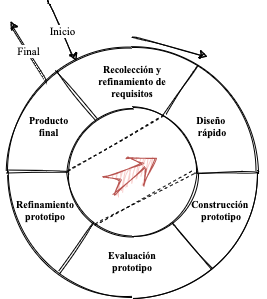
\includegraphics[width=0.3\textwidth]{cap4_analisis_tecnico/images/modelo_prototipado.png}
    \caption{Fases del modelo de prototipado \cite{modeloProtitipos}}
    \label{fig:modelo_prototipado}
\end{figure*}

Tal como se observa en la figura [\ref{fig:modelo_prototipado}], existen 6 etapas:

\begin{enumerate}
    \item \textbf{Recolección y refinamiento de requisitos}: se plantean las características que se desea que tenga el producto final: aspecto, funcionalidad, restricciones, etc. 
    \item \textbf{Diseño rápido}: se diseña el prototipo a partir de las especificaciones ofrecidas 
    \item \textbf{Construcción prototipo}: se implementa el prototipo
    \item \textbf{Evaluación prototipo}: se evalúa con los usuarios finales
    \item \textbf{Refinamiento prototipo}: se analiza el feedback y si es necesario se hacen cambios en el prototipo. En caso de que esto ocurra, se vuelve a la etapa 2 de diseño.
    \item \textbf{Producto final}: el prototipo ya está listo y se pasa a implementar el producto final.
\end{enumerate}

\subsection{Ventajas del modelo de prototipado}
Las ventajas de este modelo son las siguientes: 

\begin{itemize}
    \item Útil cuando el cliente conoce los objetivos generales para el software pero no identifica los requisitos detallados de entrada, procesamiento o salida. Permiten el desarrollo de un sistema a partir de requisitos poco claros o cambiantes.
    \item No modifica el flujo del ciclo de vida ya que hasta que se desarrolle un prototipo final no se sale de la etapa de diseño.
    \item Permite al desarrollador conocer qué desea exactamente el cliente. 
    
    \item Aumentan las probabilidades de éxito debido al constante \textit{feedback} que hay sobre el sistema; esto hace que sea improbable que el producto final no sea el esperado.
    \item Reduce el riesgo de construir productos que no satisfagan las necesidades de los usuarios porque estos están constantemente probándolo y aportando ideas de mejora de usabilidad.
    \item  Son más fáciles de abordar con los usuarios finales. Su uso redunda en una mayor satisfacción del usuario con el producto final, ya que él o ella han participado activamente de su diseño. Curva menor de aprendizaje.
    \item Permite a todos los involucrados entender bien y mejor el problema antes de la implementación final.
    \item Se reduce el riesgo o la incertidumbre sobre la implementación del software ya que antes de empezar con el producto final, el prototipo ya estará muy bien estudiado por lo que se conocerán cuáles son las necesidades de implementación.
    \item Como información complementaria a los requisitos constituyen un gran apoyo a las estimaciones de esfuerzo de todas las áreas, incluyendo proveedores.
\end{itemize}

\subsection{Desventajas del modelo de prototipado}
Las desventajas de este modelo son las siguientes: 

\begin{itemize}
    \item El cliente puede confundir el prototipo con el producto final, por ejemplo esperando que el producto ya esté listo pero en realidad ahora se empezará a construir.
    \item En la implementación el prototipo puede ser modificado y/o ampliado por sus desarrolladores sin consultar con el cliente, rompiendo así el compromiso de calidad y mantenimiento que tiene con este
    \item Adoptarlo como el sistema final: Los usuarios y profesionales de sistemas pueden considerar al prototipo como el sistema final cuando aún es incompleto e inadecuado.
    \item Los prototipos generan o pueden generar otro tipo de problemas si su presentación y discusión con los usuarios no es controlada: puesto que son modelos inconclusos, los usuarios suelen enfocarse en aspectos “superficiales” del prototipo que los pueden dejar inconformes luego de verlos por primera vez. También es posible que se pierda mucho tiempo, innecesariamente, tratando de hacer entender al usuario la finalidad real de los prototipos.
    \item Requiere participación activa del usuario, al menos, para evaluar el prototipo. Y mucho más involucramiento si queremos que participe en su creación.
    \item Una desventaja importante a tener en cuenta es la falta de experiencia que tienen muchos analistas Funcionales en programación y en actividades de diseño de interfaces de usuario.
\end{itemize}

\section{Diagrama de Gantt}

\section{Herramientas utilizadas para el desarrollo}

En este apartado se detallarán qué medios se han utilizado para la implementación de este proyecto: el lenguaje empleado, las tecnologías, las herramientas y librerías. 
\subsection{Lenguaje de programación} 

En la actualidad hay un total de 16 lenguajes distintos para el desarrollo de programas de inteligencia artificial. Para poder elegir un lenguaje es necesario analizar las características y las ventajas de cada uno de ellos y, junto con los requerimientos del proyecto, decidir qué lenguaje es el que mejor se adapta al problema. \\

Debido al elevado número de lenguajes, se han ido descartando hasta quedar con los dos lenguajes más empleados en los últimos años: \textbf{\textit{R}} y \textbf{\textit{Python}}. \\

\textbf{R} es un lenguaje altamente enfocado a la estadística, trato de datos, análisis numéricos y, por supuesto, el Aprendizaje Máquina. \\

\textbf{Python}, por otro lado, es un lenguaje que se usa en una multitud de ámbitos y consta de una gran comunidad, de un gran nombre de librerías. \\

Para la implementación del proyecto se ha elegido el lenguaje \textbf{Python} ya que:

\begin{itemize}
    \item Es \textbf{\textit{fácil de utilizar}} y el código resultante es \textbf{\textit{muy comprensible}}
    \item \textbf{\textit{Gran número de librerías}} que implementan partes de código necesarios y que, además, supondría una carga añadida si fuese necesario programarlo. En la siguiente sección se concretarán las librerías empleadas.  
    \item \textbf{\textit{Comunidad extensa}} y muy implicada, por lo que muchas dudas que puedan surgir a la hora de la implementación es probable que ya esté resuelta si se busca 
\end{itemize}

\subsection{Librerías} 

La librería más importante utilizada es la de \textbf{\textit{Gym}}, librería utilizada para poder crear el entorno del agente. Dicha librería dispone de una multitud de ejemplos de entorno con características distintas. \\

Por otro lado, para poder implementar la red neuronal (es decir, el agente inteligente) se han utilizado las librerías de \textbf{\textit{Keras}} y \textbf{\textit{Tensorflow}}, que contienen todos los elementos y algoritmos necesarios. \\

Por último, se ha utilizado las librerías de \textbf{\textit{numpy}} y \textbf{\textit{pandas}} para el trato de los datos y la librería de \textbf{\textit{matplotlib}} para poder crear los gráficos. 

\subsection{Software y otros elementos} 

En cuanto a los programas utilizados, se ha empleado el programa \textbf{PyCharm} de JetBrains ya que es en IDE atractivo, fácil de usar, con integración de GIT, visualización de gráficos, visualización de bases de datos, debugger fácil, etc. \\

También se ha empleado la herramienta \textbf{Git} para el control de versiones del proyecto. 

\section{Requisitos funcionales}

Este proyecto no consta de requerimientos funcionales ya que el sistema no se espera que tenga unos resultados en concreto ni ofrezca un servicio en particular, sino que se trata de una \textbf{experimentación} con la que se llegará a unas conclusiones al cabo de su realización; por lo que, a priori, no es sencillo predecir qué resultados se obtendrán. 
\section{Requisitos no funcionales}

En cuanto a los requisitos funcionales, se tiene: 

\begin{enumerate}
    \item Emplear Reinforcement Learning
    \item Utilizar la librería \textbf{Gym} de Open AI para diseñar el entorno 
    \item Utilizar una DNN (Deep Neural Network) 
    \item Que el agente tenga la capacidad de tomar las decisiones por si mismo y que vaya aprendiendo, no que tenga un sistema de condiciones por detrás que determinen las acciones que debe tomar
\end{enumerate}

\section{Objetivos}

El objetivo principal de este proyecto es estudiar la capacidad de un agente de aprender a llegar a una casilla en concreto dentro de una matriz después de presentarle con distintas situaciones en las que ha interactuado con el entorno. 

En cuanto a objetivos más concretos, se quiere:

\begin{enumerate}
    \item Crear un entorno estático y un entorno dinámico para poder presentarle al agente la aleatoriedad de los elementos que percibe y así pueda entrenar bajo condiciones variadas. Por ejemplo, cambio de la meta o del origen, deshabilitación de casillas, etc. 
    
    \item Crear varios modelos para el agente y analizar los datos que genera: media de pasos dados para llegar a la meta, desviación típica de los pasos, error total realizado con los pasos, etc. 
    
    \item Encontrar una configuración de DNN, mínimo de 3 capas, que permita alcanzar una solución con una desviación típica menor a 3. 
    
\end{enumerate}